\section{Content of enclosed CD}
\label{appendix:cd-contents}


    \begin{enumerate}
    \item $/documents/$ - Documents which were made during the Master thesis
    \item $/evaluation/$ - Raw data of the field study, including audio recordings of all interviews and the questionnaire logs.

    \item $/misc/$ - Screenshots, photos and other files for this work.
    \item $/papers/$ - All scientific articles read for this thesis.
    \item $/presentation/$ - Presentations `Antrittsvortrag' and `Abschlussvortrag' (held in German).

    \item $/repository/$ - A copy of the GitHub repository including all development files.

    \item $/thesis/$ - LaTeX version of the thesis.

    \end{enumerate}

  \textit{PDSurvey}'s source code and documentation can also be found in the following GitHub repository: \url{https://github.com/lukasziegler/masterarbeit/tree/master/docs}



%% - - - -  P A P E R S   R E A D  - - - - %%
\cleardoublepage
\section{Evaluation of Public Displays}
\label{appendix:evaluation-of-PDs}

  Reasons stated in the semi-structured interviews for and against each feedback channel. \\


        % 1) TV SCREEN
  \begin{table}[h]
    \small
    \center

    \begin{tabular}{p{7cm}p{7cm}}
    \toprule
    \textbf{Pro ``TV Screen''}  &  \textbf{Contra ``TV Screen''} \\ \midrule

    4x Most direct, immediate feedback  &  4x Display is too large  \\
    2x I am already standing here (2x)  &  3x Feels too public  \\
    1x Seems easiest  &  2x Everyone could watch me  \\
    1x Requires less personal information  &  1x That is mean, when the screen is so large  \\
    1x All on one device  &  1x The keyboard on the display would have been too large and confusing  \\
    1x I can use it without putting my glasses on  &  1x Display is uncomfortable for reading long questions  \\
    1x Seems to be the fastest option  &  1x Don't feel comfortable standing in focus in such a large room  \\

      &  1x The system is too innovative, that is why I wouldn't trust it yet \\
      &  1x Because of social desirability influencing my responses  \\

    \bottomrule
    \end{tabular}

    \caption[Feedback Channel - TV Screen]{Reasons mentioned for/against using the \textit{TV screen} as a feedback channel.}
    \label{table:feedback-channel-TV-screen}
  \end{table}

 

  % 2) TABLET

  \begin{table}[h]
    \small
    \center

    \begin{tabular}{p{7cm}p{7cm}}
    \toprule
    \textbf{Pro ``Tablet''}  &  \textbf{Contra ``Tablet''} \\ \midrule
    5x The display is smaller and better laid out)  &  2x Redundancy (``why do I need a tablet when I can respond on the TV screen?'') \\
    2x Better sensitivity / user experience  &  1x Personal aversion (he had bad experiences with tablets) \\
    2x It feels more private  &   \\
    1x Because it is its sole purpose  &   \\
    1x You are not in the way of others  &   \\
    1x I am more used to it  &   \\
    1x Most interactive option  &   \\
    1x Less people watching  &   \\
    1x Because I expect a better input  &   \\
    1x Requires less personal information  &   \\
    1x More comfortable standing here  &   \\
    \bottomrule
    \end{tabular}

    \caption[Feedback Channel - Tablet]{Reasons mentioned for/against using the \textit{Tablet} as a feedback channel.}
    \label{table:feedback-channel-tablet}
  \end{table}




  % 3) SMARTPHONE

  \begin{table}[h]
    \small
    \center

    \begin{tabular}{p{7cm}p{7cm}}
    \toprule
    \textbf{Pro ``Smartphone''}  &  \textbf{Contra ``Smartphone''} \\ \midrule

    1x I use it most often  &  4x Too much effort \\
    1x It belongs to me  &  3x Too indirect \\
      &  3x Requires more personal information \\
      & 2x I am not sure how complex and time-consuming it would be to set it up \\
      &  1x I don't know if I would know how to do it \\
      &  1x Too small display for comfortably answering surveys and long questions \\
      &  1x Too cumbersome \\
      &  1x I would assume that I would have to install some sort of software \\
      &  1x Privacy \\

    \bottomrule
    \end{tabular}

    \caption[Feedback Channel - Smartphone]{Reasons mentioned for/against using the \textit{Smartphone} as a feedback channel.}
    \label{table:feedback-channel-smartphone}
  \end{table}


  % 4) EMAIL

  \begin{table}[h]
    \small
    \center

    \begin{tabular}{p{7cm}p{7cm}}
    \toprule
    \textbf{Pro ``Email''}  &  \textbf{Contra ``Email''} \\ \midrule

    4x I can do it at home  &  5x I would forget about it  \\
    3x I have more time to complete the survey  &  4x I don't like to submit my email address  \\
    1x Better warranty of privacy  &  3x I don't like to postpone it  \\
    1x I could deliver qualitatively better results  &  2x It would take too long to complete  \\
    1x I wasn't sure which kind of questions to expect  &  2x Too much effort  \\
      &  1x Requires more personal information  \\
      &  1x Too indirect  \\

    \bottomrule
    \end{tabular}

    \caption[Feedback Channel - Email]{Reasons mentioned for/against using the \textit{Email} as a feedback channel.}
    \label{table:feedback-channel-email}
  \end{table}



%% - - - I N T E R V I E W S   C A R R I E D   O U T  - - - %%
\clearpage

\label{appendix:interviews}

  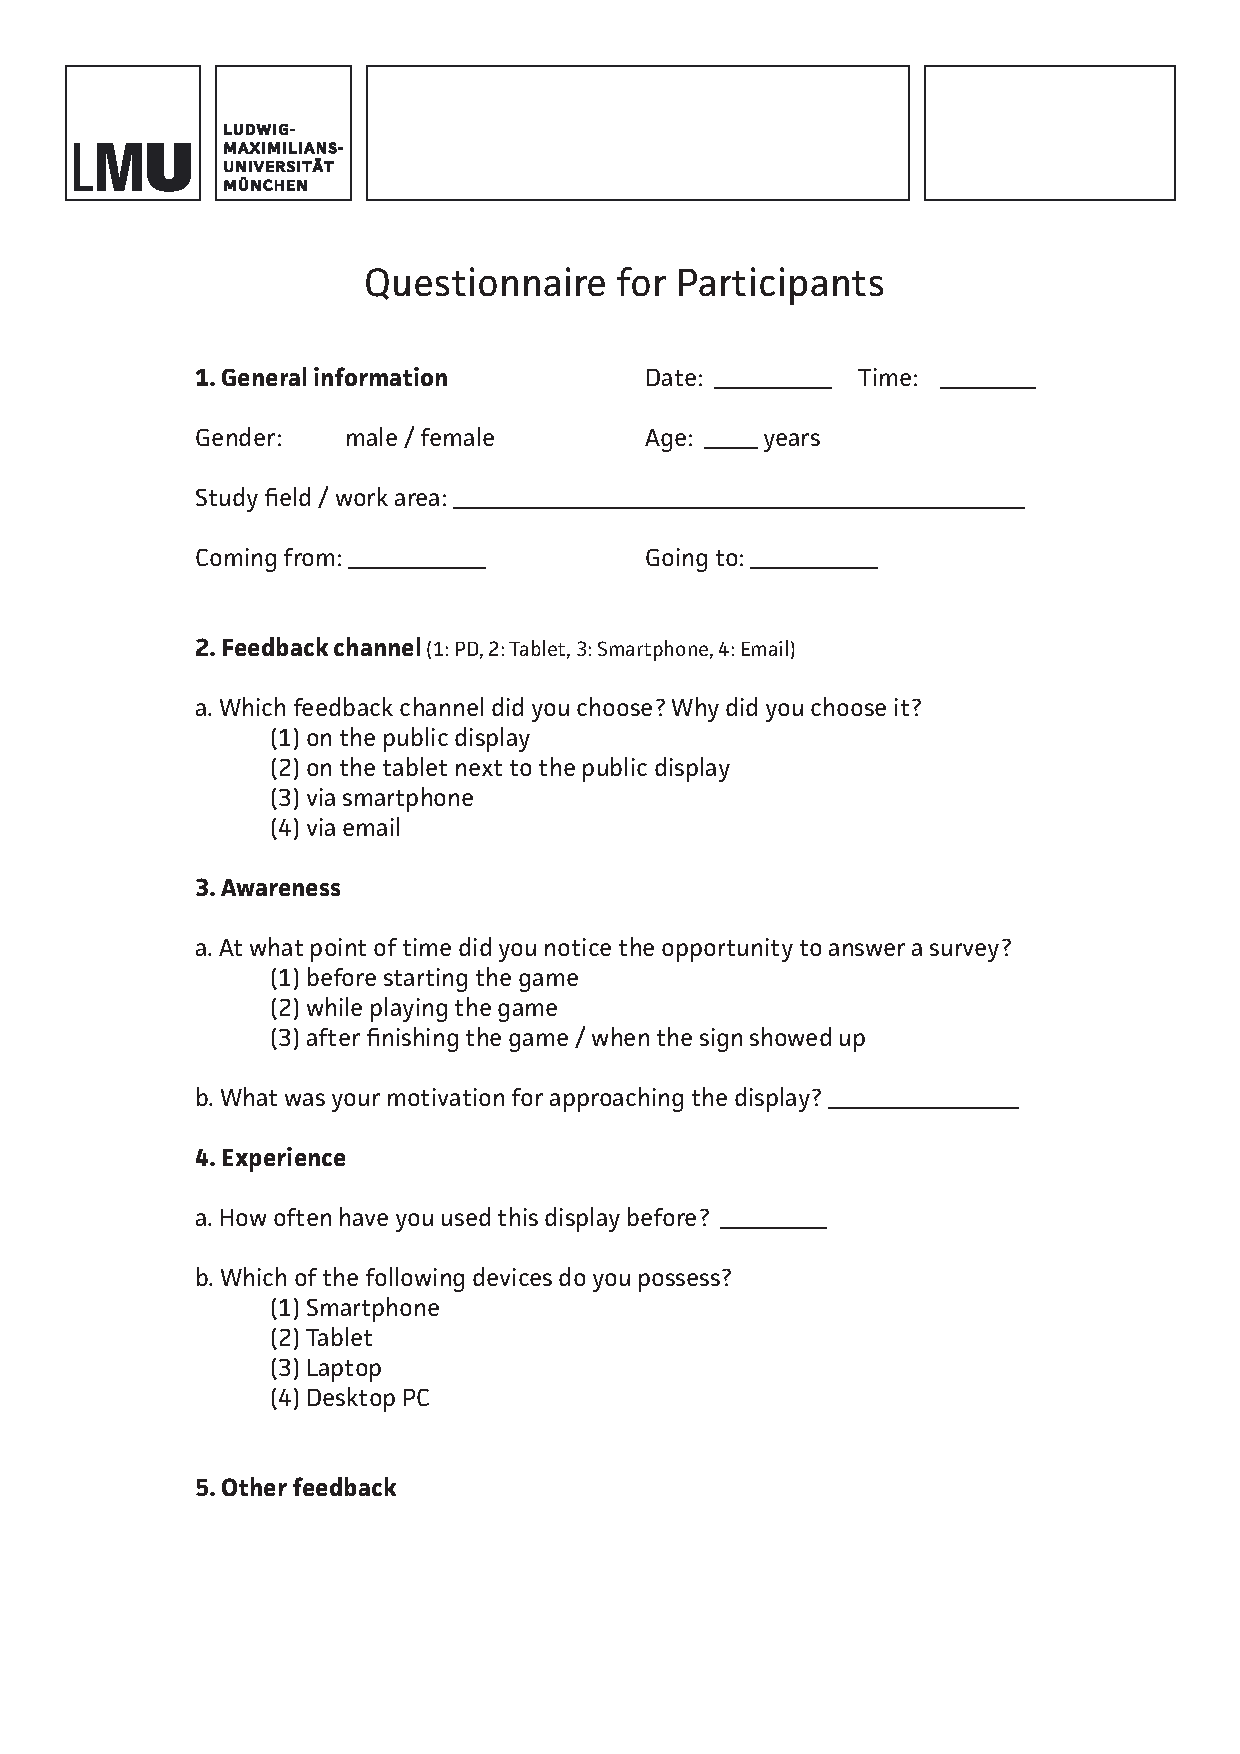
\includepdf[pages={-},scale=.9,offset=0 -50,pagecommand=\section{Questionnaires for Field Study}]{pdf/interview-participants.pdf}
  \label{appendix:interview-participant}

  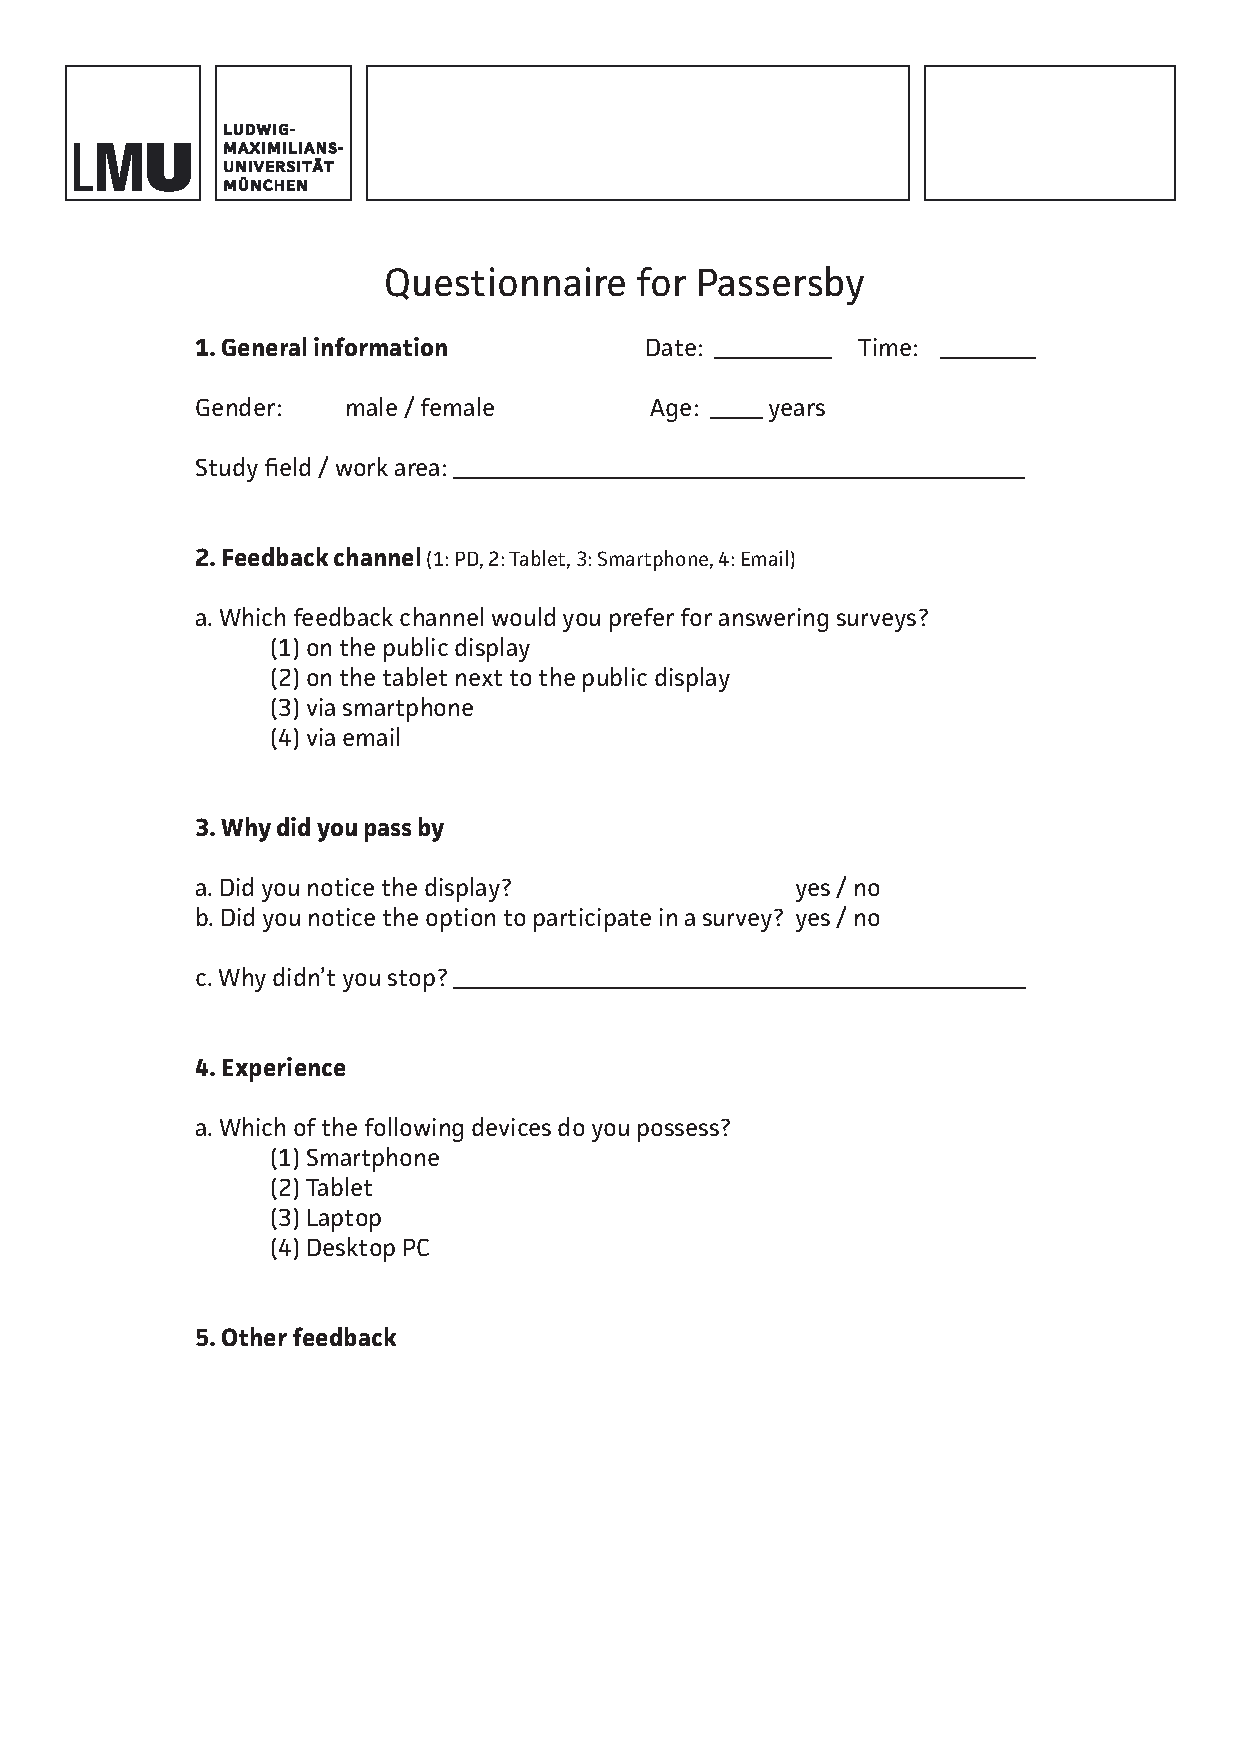
\includepdf[pages={-},scale=.9, offset=0 -25,pagecommand={}]{pdf/interview-passersby.pdf}
  \label{appendix:interview-passerby}

  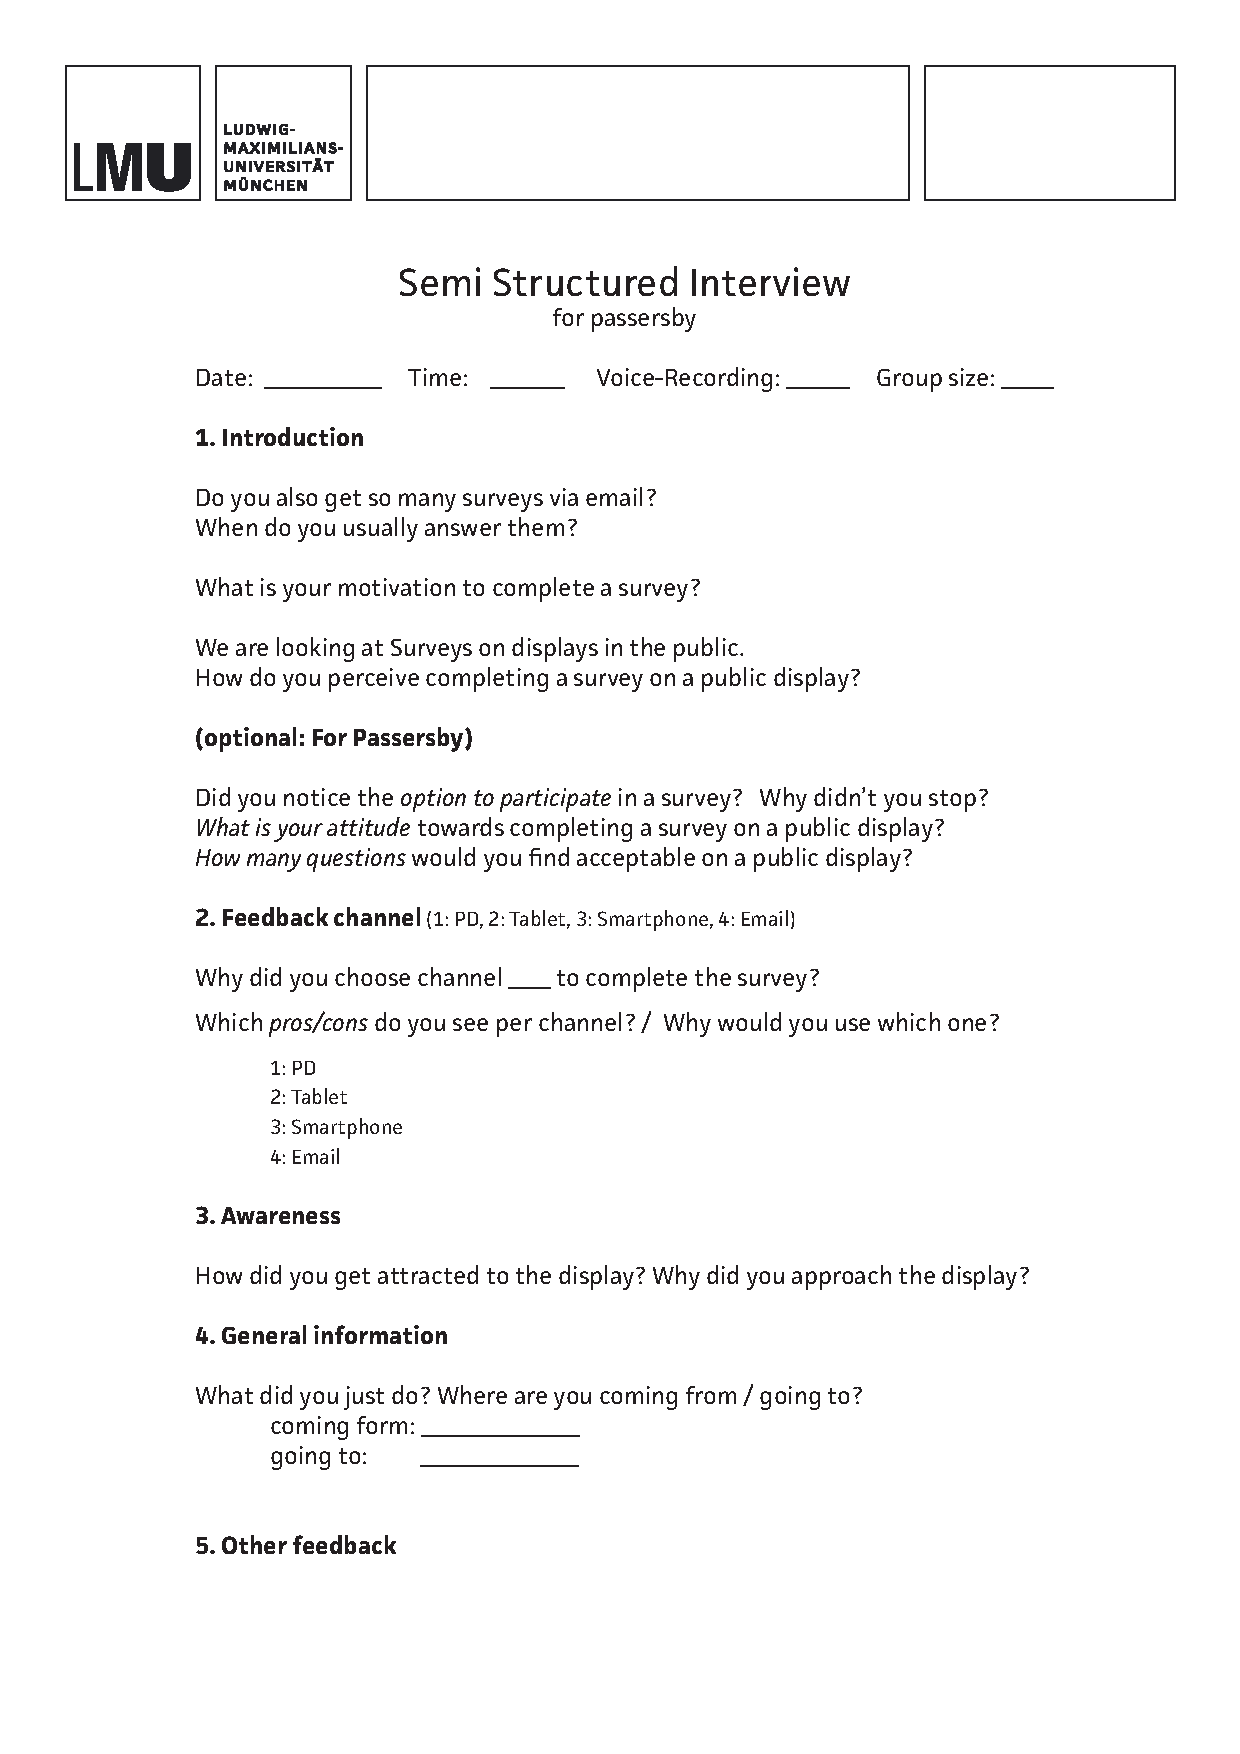
\includepdf[pages={-},scale=.9, offset=0 -25,pagecommand={}]{pdf/semi-structured-interview.pdf}
  \label{appendix:semi-structured-interview}





%% - - - - S C R E E N S H O T S - - - - %%
\cleardoublepage
\section{Screenshots of Platform}



\paragraph{Balloon Shooter Game}


\label{appendix:screenshots-balloon-shooter}

The following screenshots originate from the Balloon Shooter game developed by Jiamin Shi.
Each user first saw the options panel (see figure \ref{screenshot:options}) after completing a game of Balloon Shooter. Four channels were offered for completing the questionnaire. The order was randomized. \\




   \begin{figure}[hb]
        \centering
        \begin{subfigure}{0.7\textwidth}
            \centering
        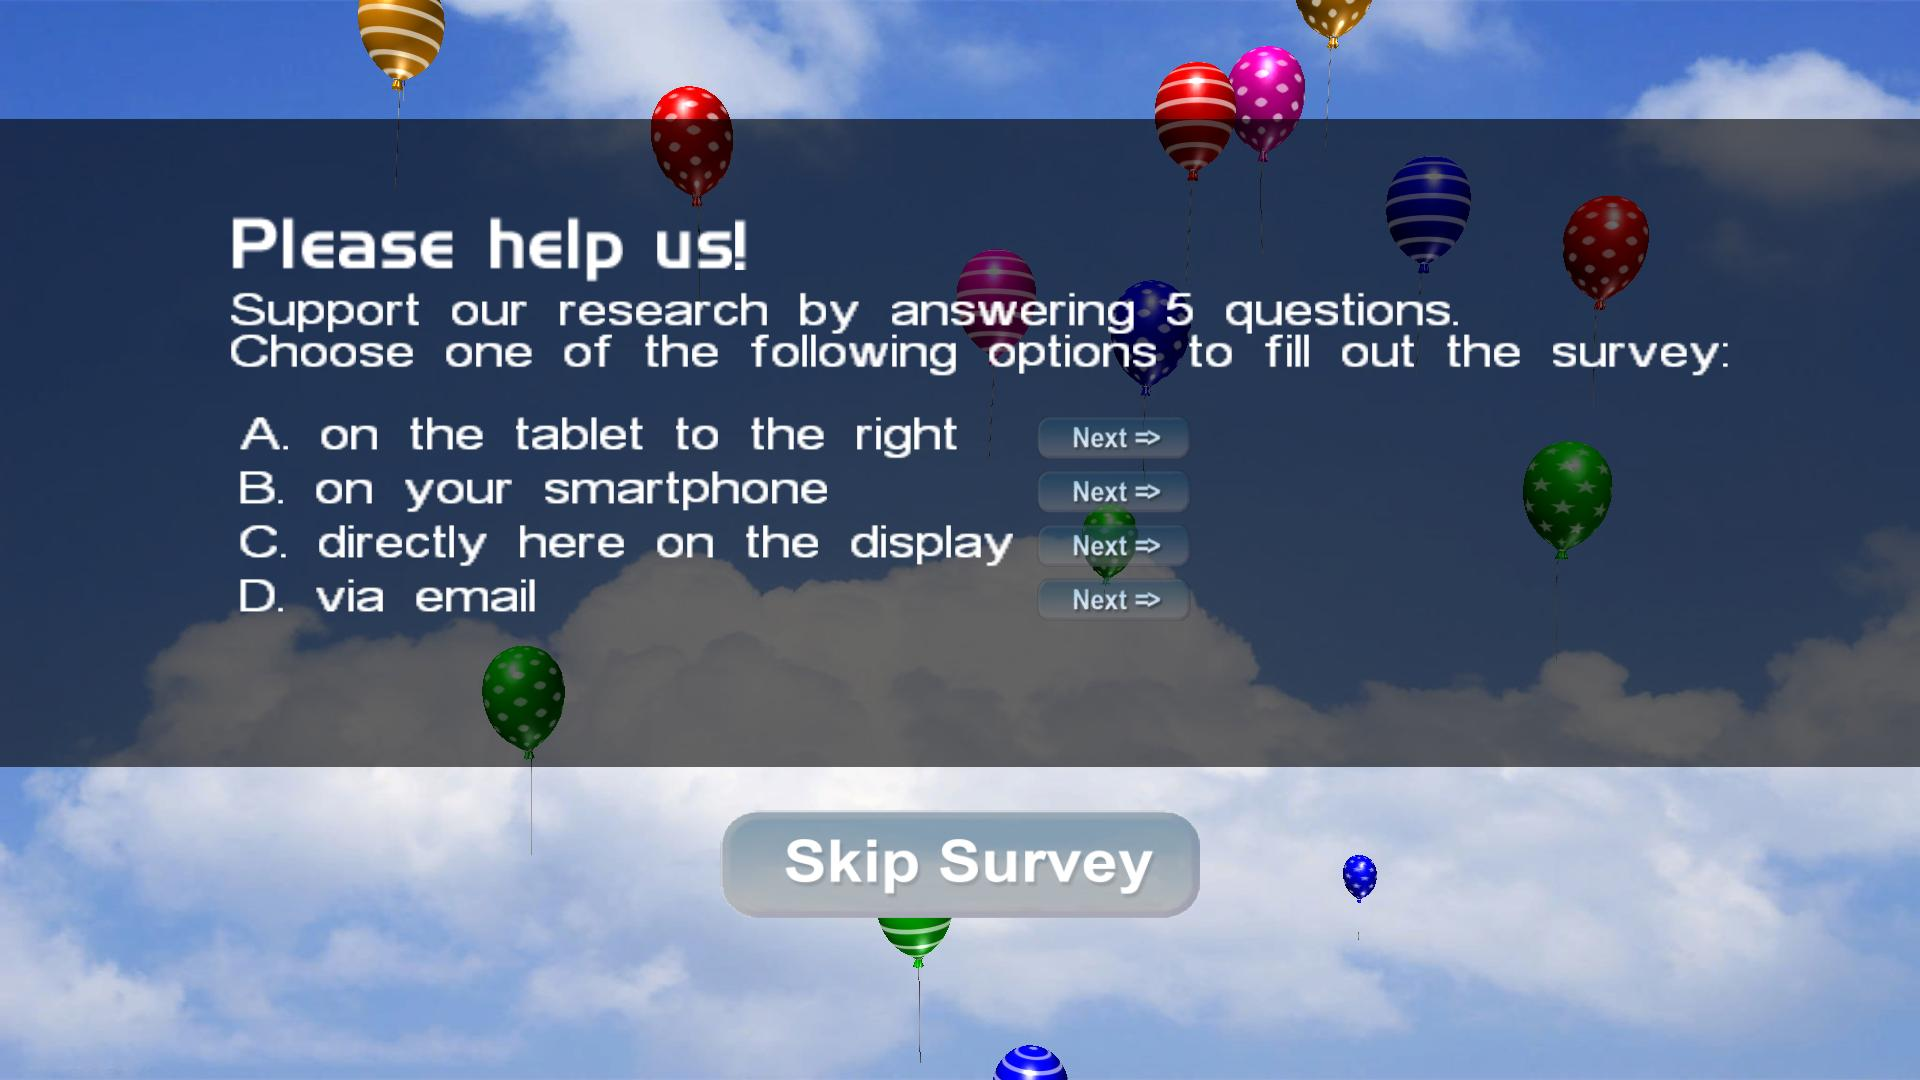
\includegraphics[width=\columnwidth]{img/screenshots/balloon-game/options-overview.jpg}
            \caption{\textbf{Options panel} - Four feedback channels are offered in a randomized order for responding to the questionnaire. \\}
            \label{screenshot:options}
        \end{subfigure}
        \hfill
        \begin{subfigure}{0.7\textwidth}
            \centering
    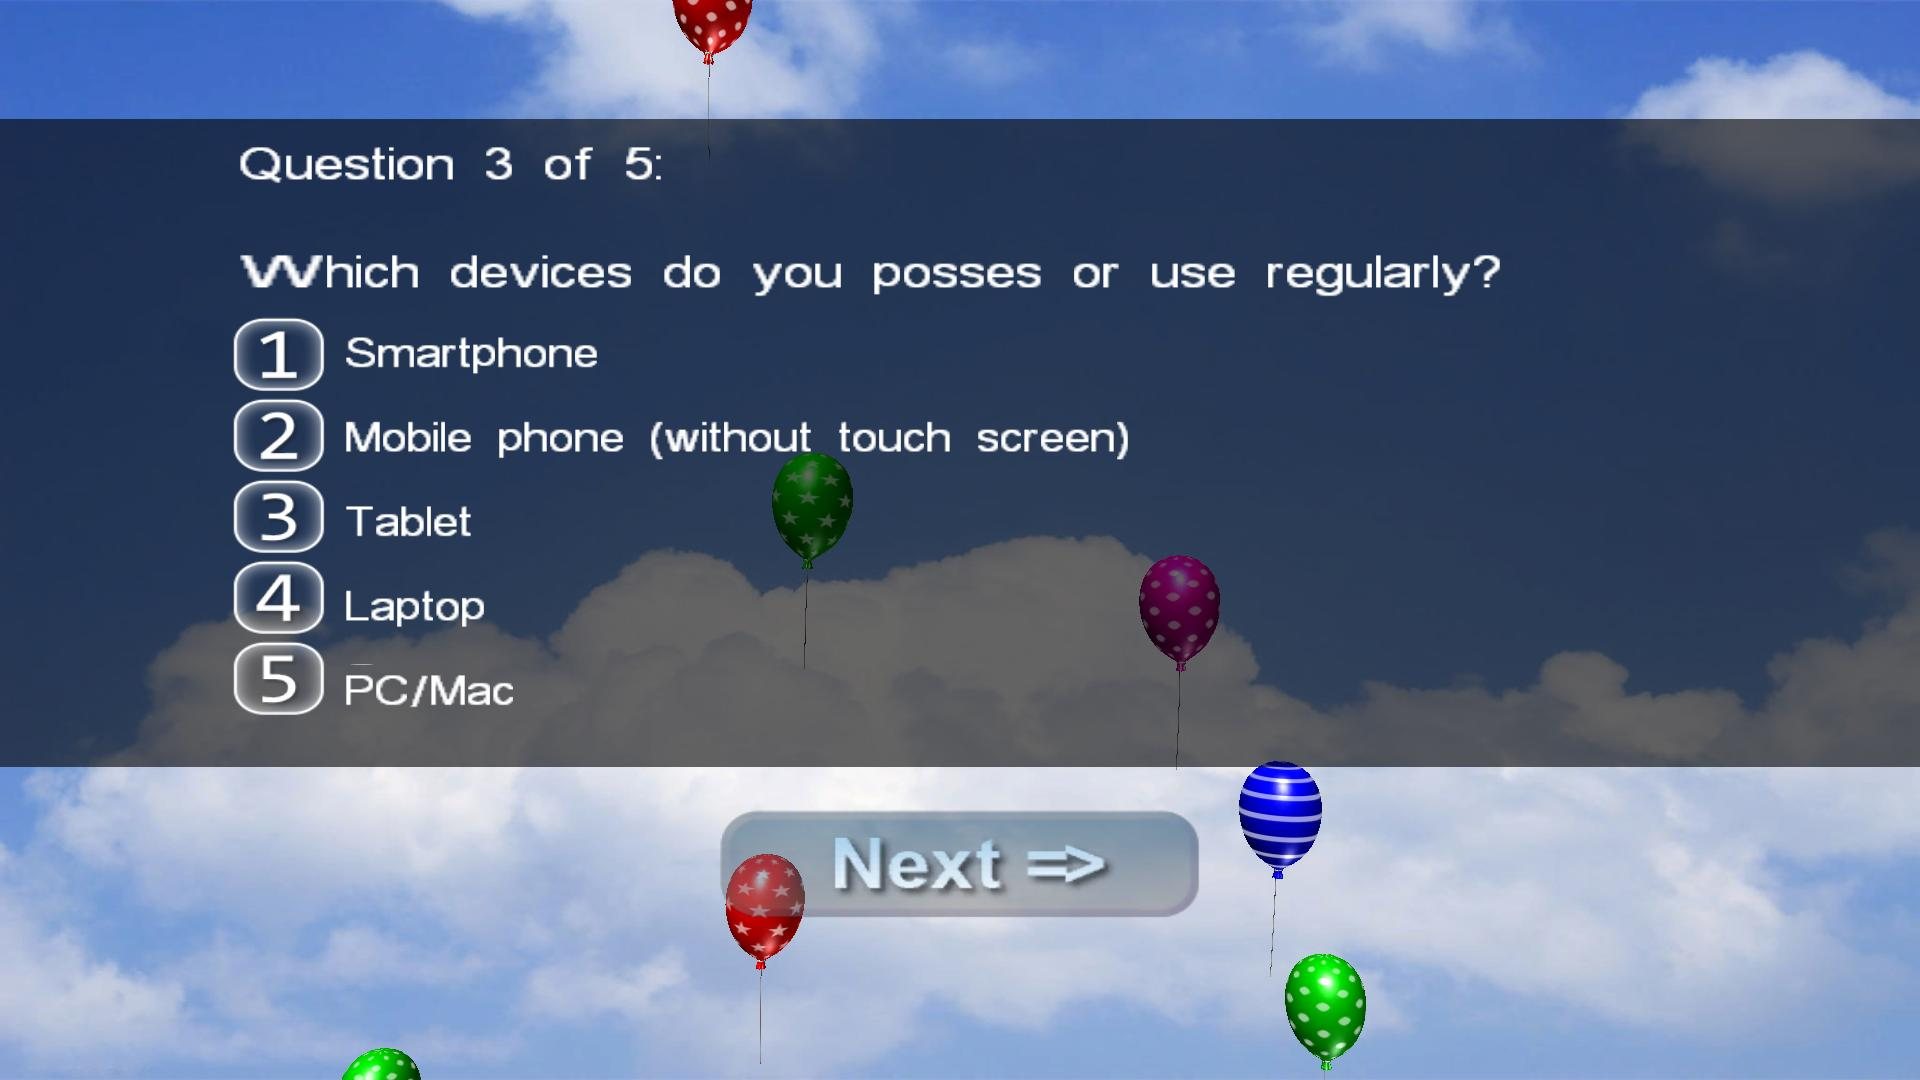
\includegraphics[width=\columnwidth]{img/screenshots/balloon-game/option-tv.jpg}
            \caption{\textbf{TV Screen option} - directly answering on the TV screen. Here you see a sample question getting asked on the interactive display. \\}
            \label{screenshot:tv-option}
        \end{subfigure}
    \end{figure}





    \begin{figure}
        \centering
        \begin{subfigure}[b]{0.7\textwidth}
            \centering
            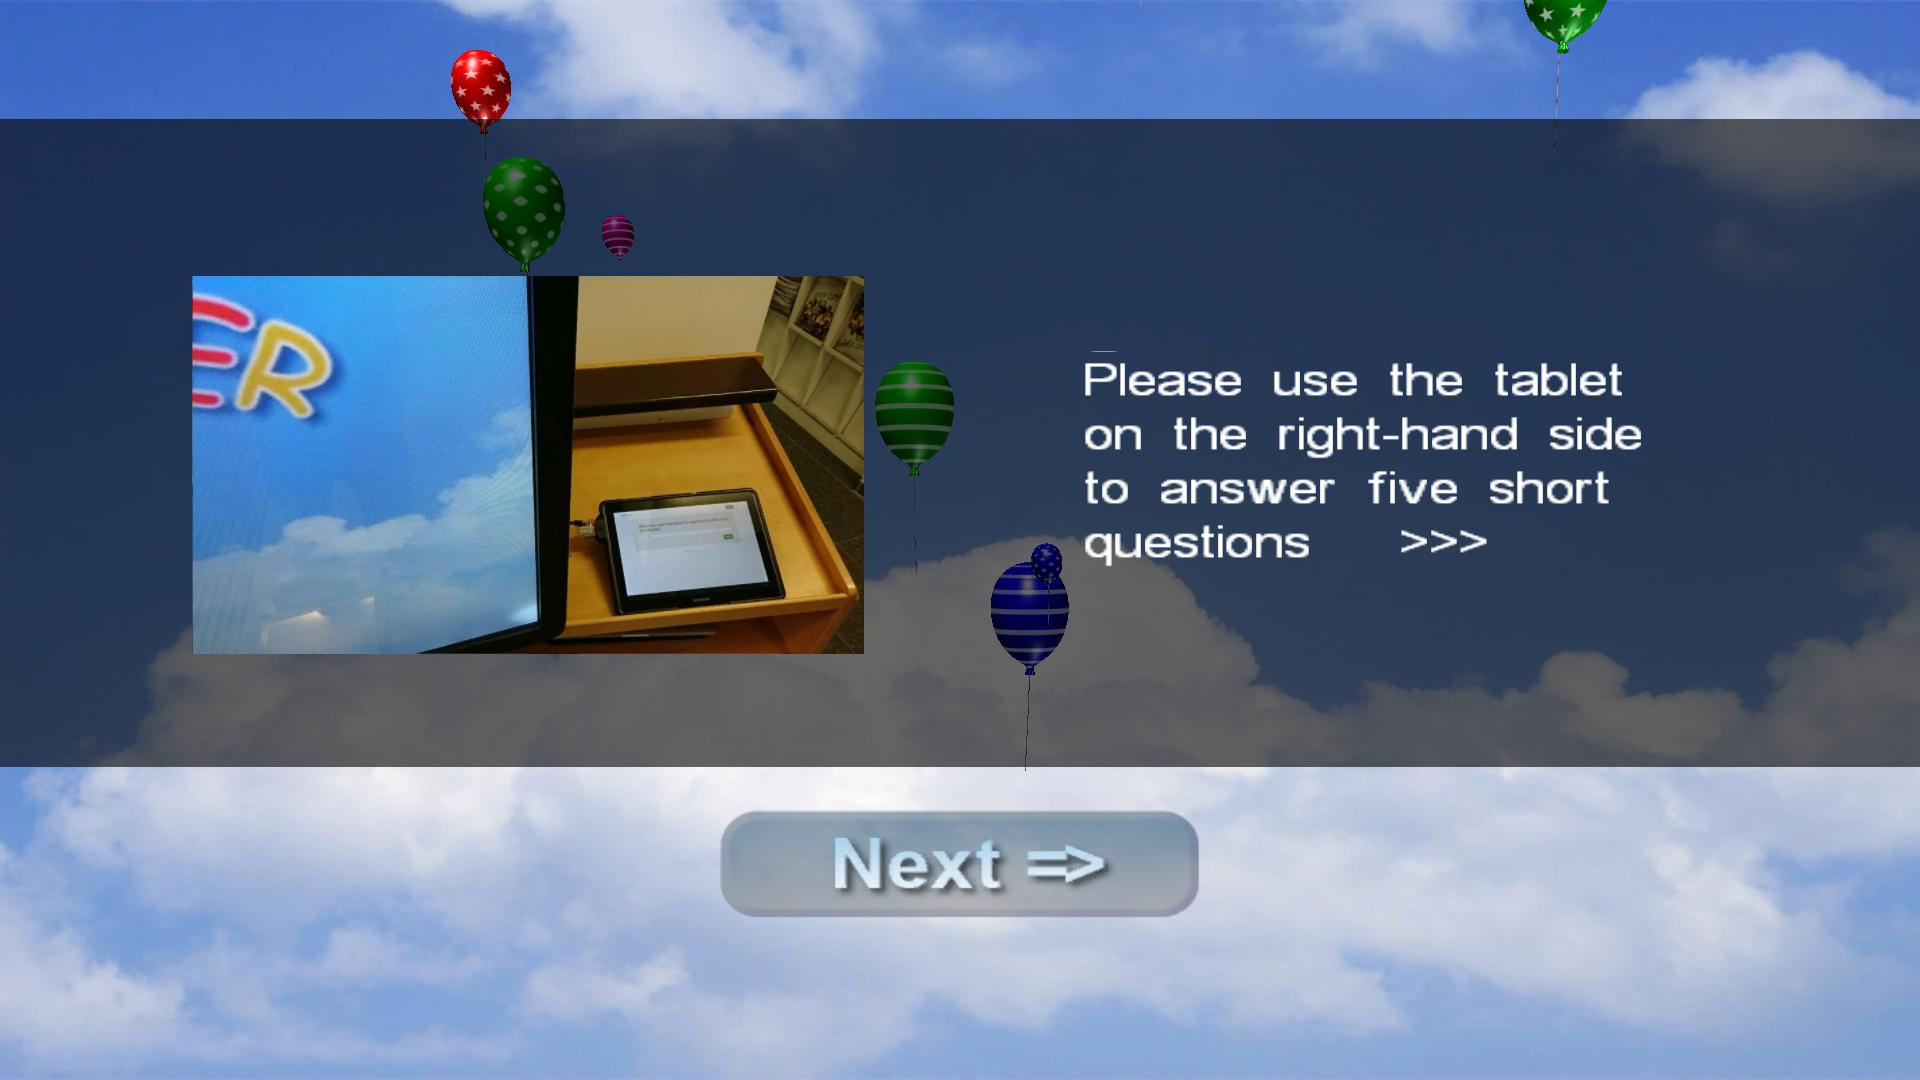
\includegraphics[width=\columnwidth]{img/screenshots/balloon-game/option-tablet.jpg}
            \caption{\textbf{Tablet option} - The screen the user sees when choosing to complete the survey on the tablet. \\}
            \label{screenshot:tablet-option}
        \end{subfigure}
        \hfill
        \begin{subfigure}[b]{0.7\textwidth}
            \centering
            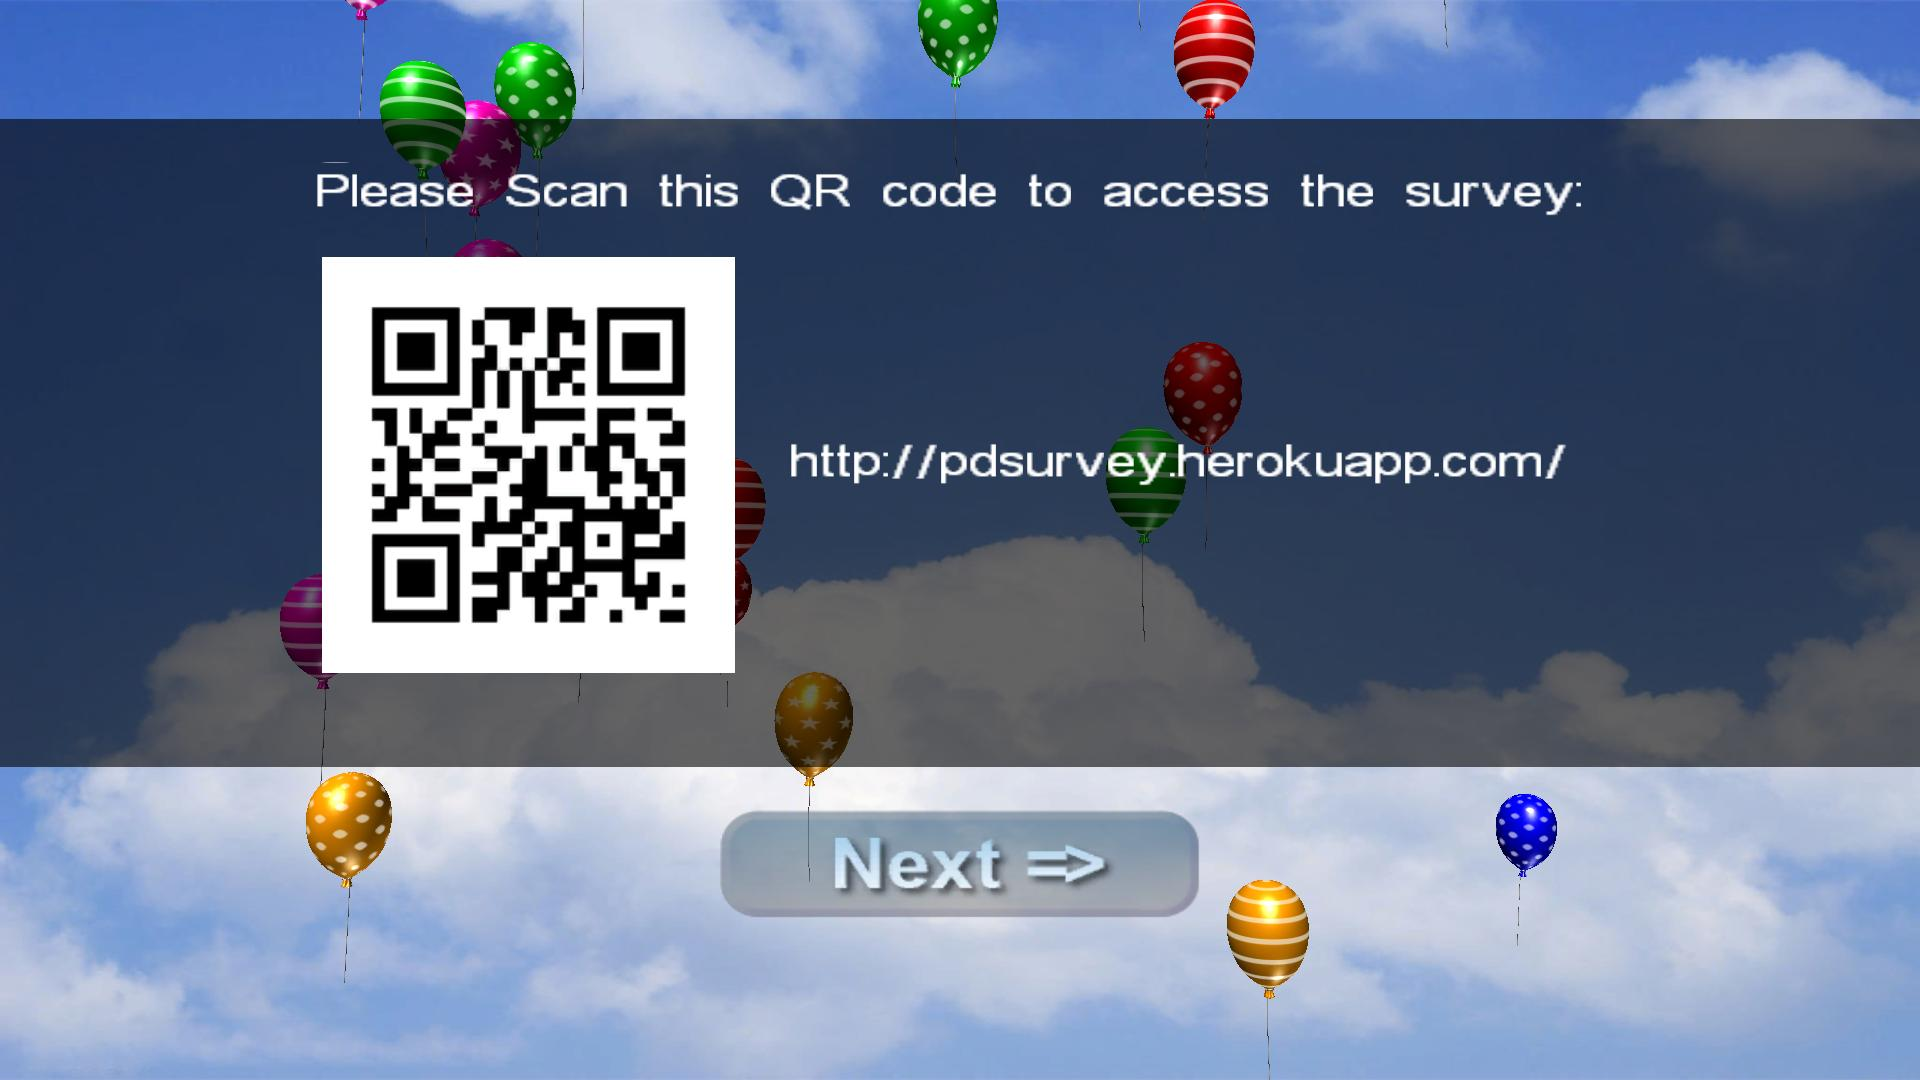
\includegraphics[width=\columnwidth]{img/screenshots/balloon-game/option-smartphone.jpg}
            \caption{\textbf{Smartphone option} - participating with your own smartphone, either by scanning the QR code or by typing the URL in the mobile browser. \\}
            \label{screenshot:smartphone-option}
        \end{subfigure}
        \hfill
        \begin{subfigure}[b]{0.7\textwidth}
            \centering
    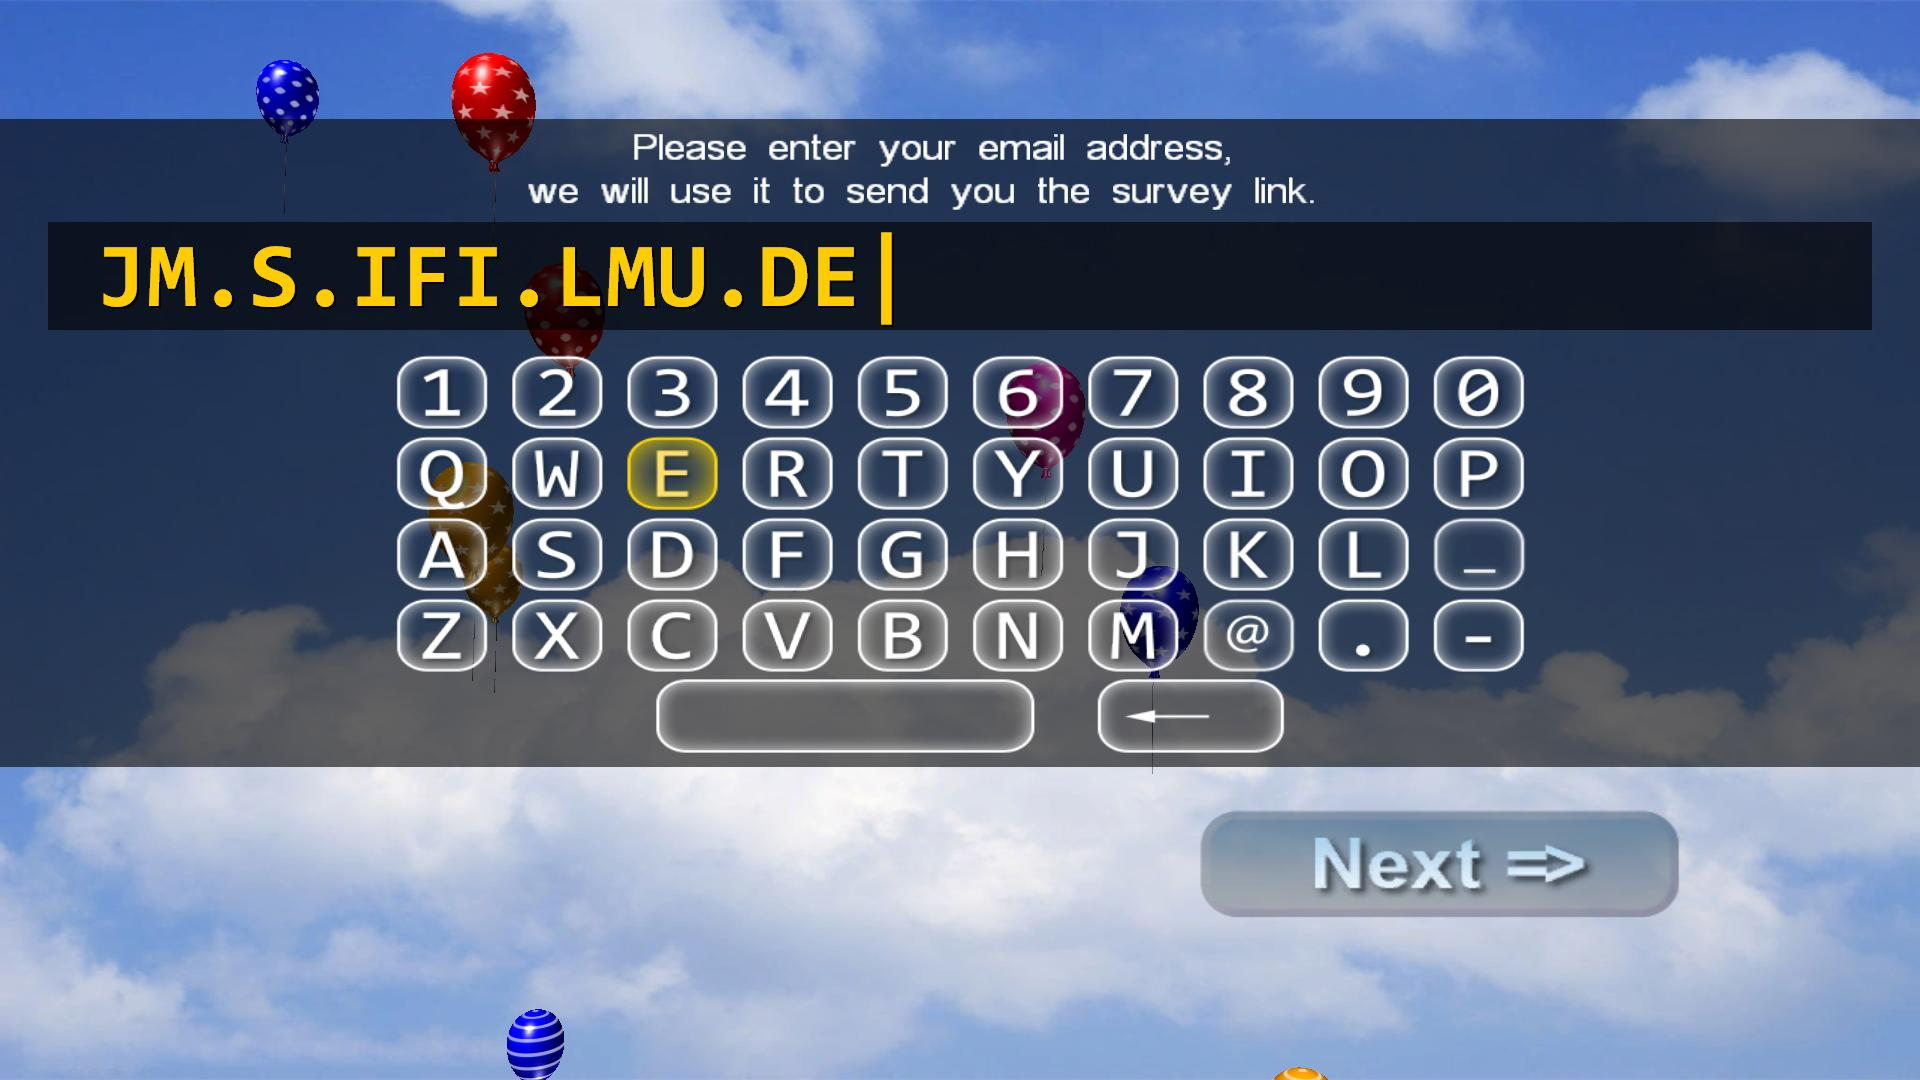
\includegraphics[width=\columnwidth]{img/screenshots/balloon-game/option-email.jpg}
            \caption{\textbf{Email option} - submitting ones email address and getting the survey link to participate in response.}
            \label{screenshot:email-option}
        \end{subfigure}
        \caption{Further screenshots from PDAdmin}
    \end{figure}




\clearpage

\paragraph{PDAdmin}

    \begin{figure}[h]
        \centering
        \begin{subfigure}{0.55\textwidth}
            \centering
            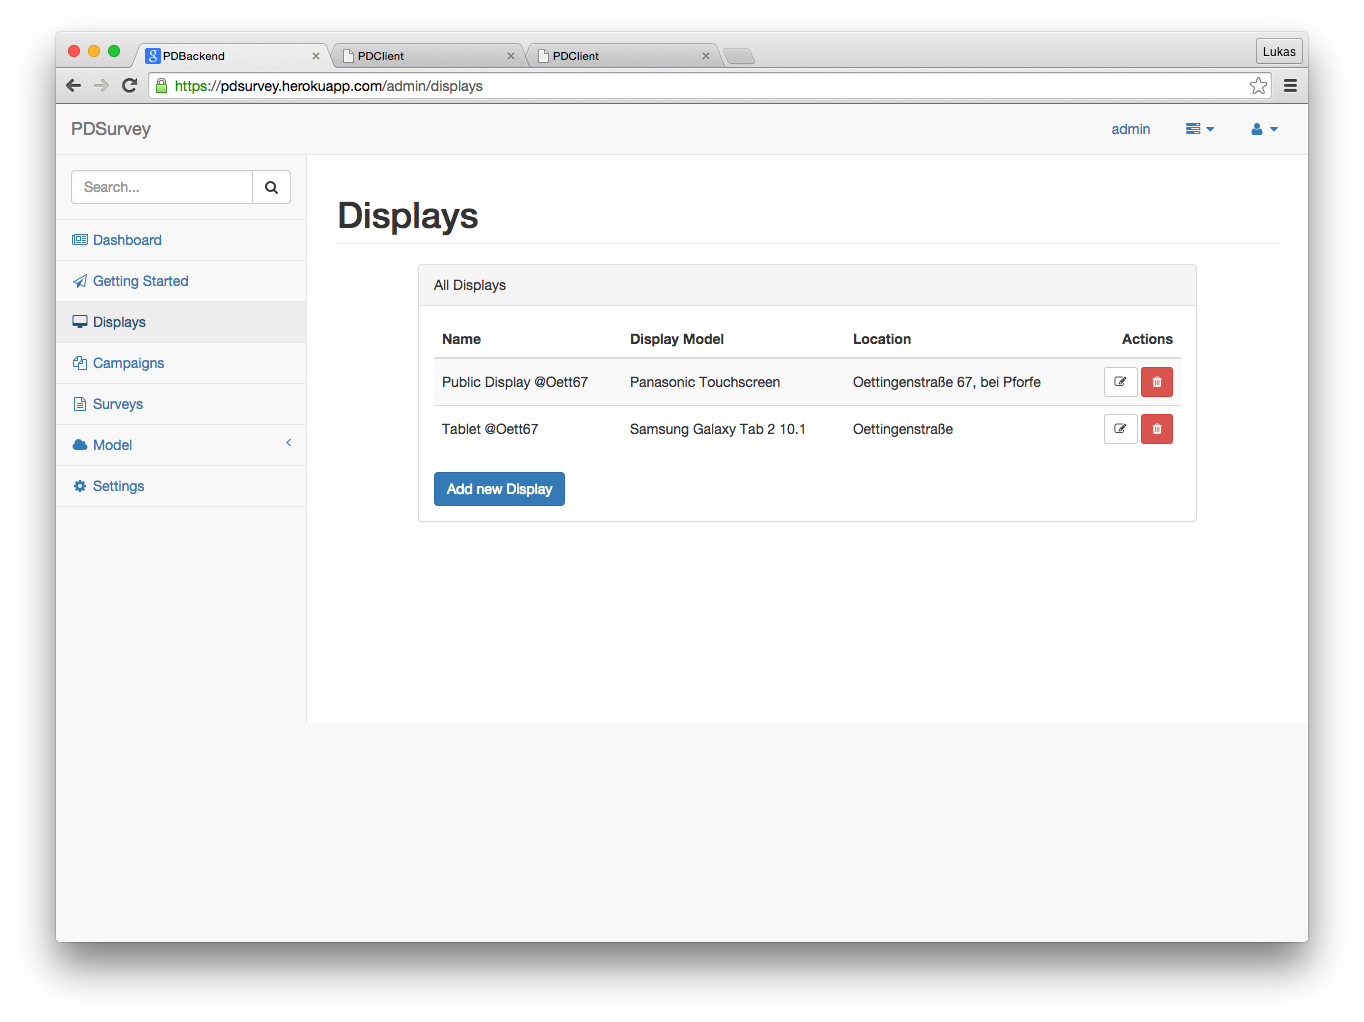
\includegraphics[width=\columnwidth]{img/screenshots/pdadmin/displays.png}
            \caption{Displays list view}
            \label{screenshot:pdadmin-displays}
        \end{subfigure}
        \hfill
        \begin{subfigure}{0.55\textwidth}
            \centering
            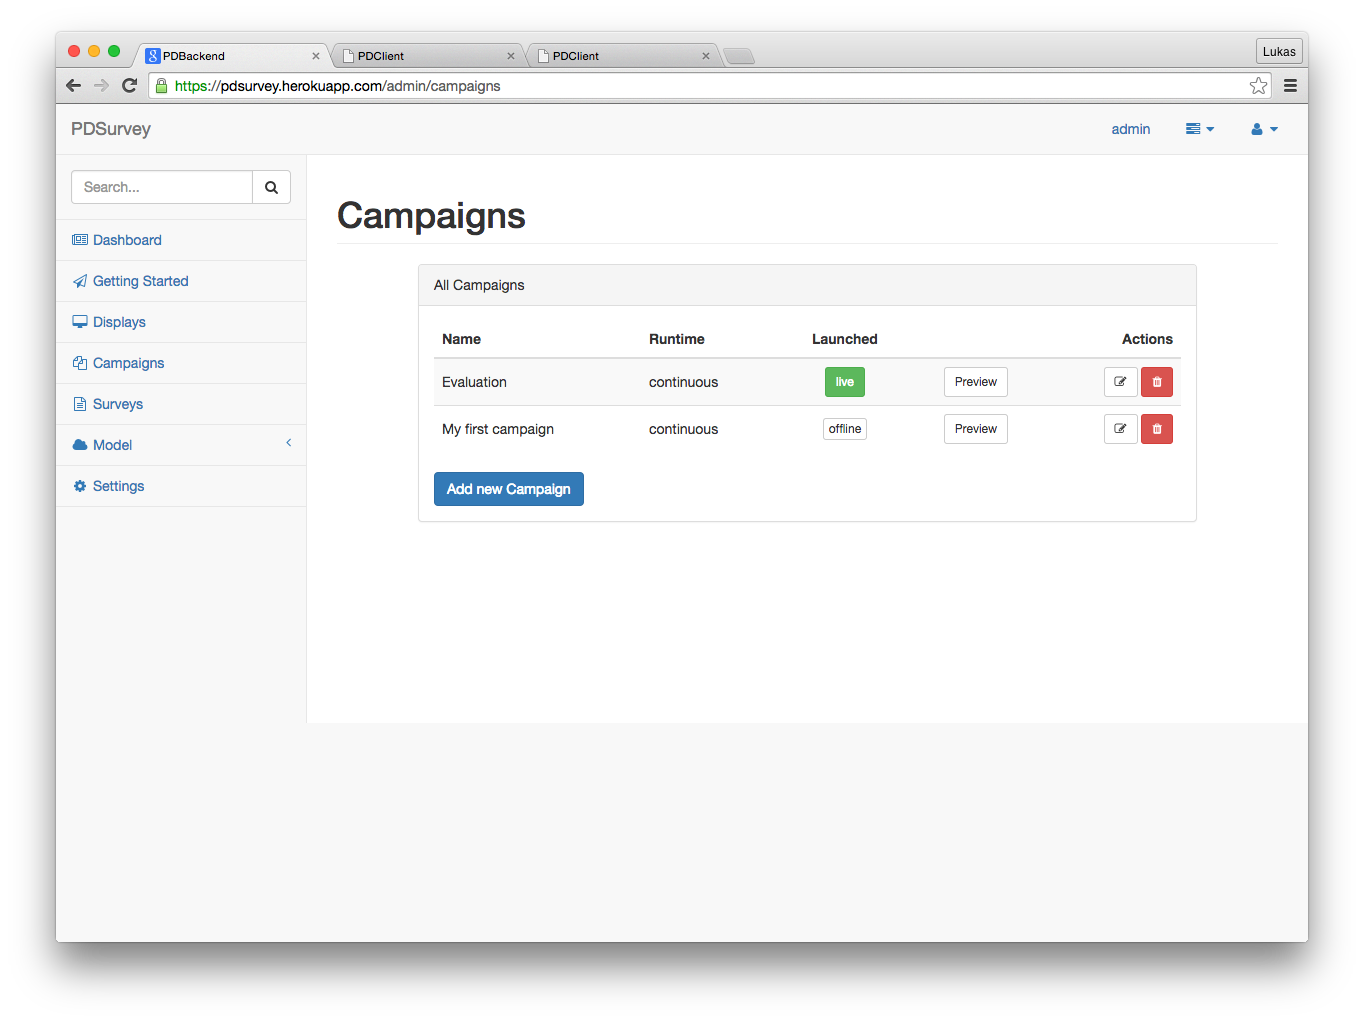
\includegraphics[width=\columnwidth]{img/screenshots/pdadmin/campaigns.png}
            \caption{Campaigns list view}
            \label{screenshot:pdadmin-campaigns}
        \end{subfigure}
        \hfill
        \begin{subfigure}{0.55\textwidth}
            \centering
            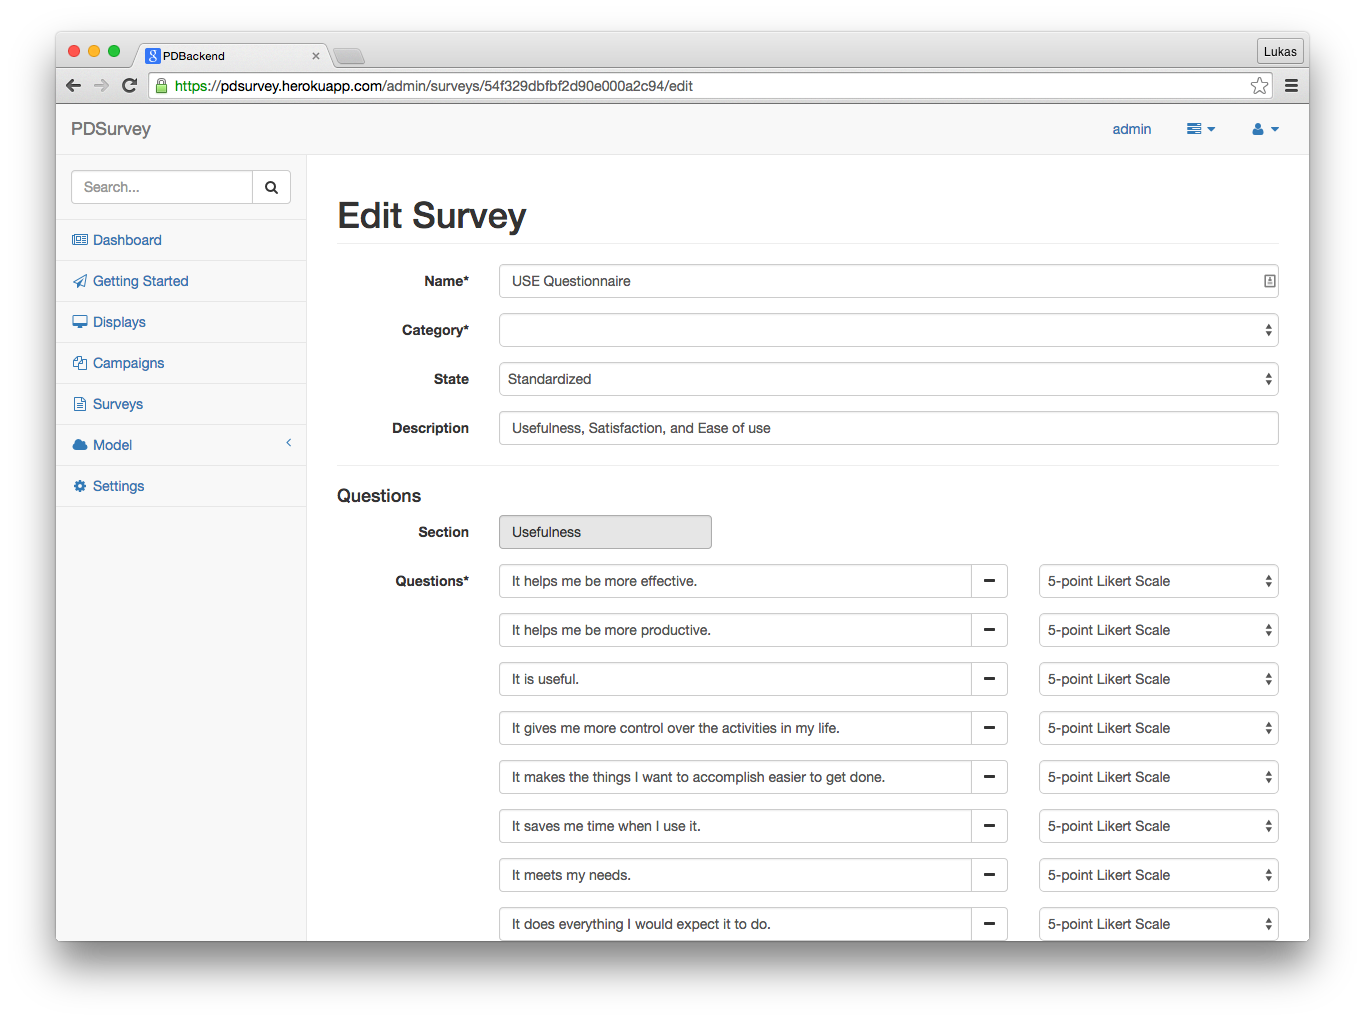
\includegraphics[width=\columnwidth]{img/screenshots/pdadmin/surveys.png}
            \caption{Survey edit page}
            \label{screenshot:pdadmin-surveys}
        \end{subfigure}
        \caption{Further screenshots from PDAdmin}
    \end{figure}


